%! Author = Juniell
%! Date = 05.05.2021

% Preamble
\documentclass[a4paper, 14pt]{extarticle}

% Packages
\usepackage[T2A]{fontenc}
\usepackage{natbib}
\usepackage{graphicx}
\usepackage[english, russian]{babel}
\usepackage{fontspec}
\usepackage{amsmath}
\usepackage{amsfonts}
\usepackage{amssymb}
\usepackage{amsthm}
\usepackage{mathtools}
\usepackage{mathrsfs}
\usepackage{fullpage}
\usepackage{ulem}
\usepackage{setspace}
\usepackage{listings}
\usepackage{indentfirst}
\usepackage[left=2cm,right=1.5cm,top=2cm,bottom=2cm]{geometry}
\usepackage{xcolor}
\usepackage{float}
\usepackage{csquotes}
\usepackage{hyperref}
\usepackage{graphics}

\definecolor{urlcolor}{HTML}{0000FF} % цвет ссылок
\definecolor{linkcolor}{HTML}{000000} % цвет гиперссылок
\hypersetup{pdfstartview=FitH, linkcolor=linkcolor, urlcolor=urlcolor, colorlinks=true}

\setmainfont{Times New Roman}
\setlength{\parindent}{5ex}
\setlength{\parskip}{1em}
\renewcommand{\baselinestretch}{1}

\graphicspath{{resources/Images}}

\definecolor{buzzlightyear}{HTML}{8757A5}
\definecolor{grass}{HTML}{738D06}
\definecolor{literal}{HTML}{F18A2B}
\definecolor{commentcolor}{HTML}{8E908B}

\lstdefinestyle{habrstyle}{
    backgroundcolor=\color{white},
    commentstyle=\color{commentcolor},
    keywordstyle=\bfseries\color{buzzlightyear},
    numberstyle=\tiny\color{commentcolor},
    stringstyle=\color{grass},
    basicstyle=\ttfamily\footnotesize,
    breakatwhitespace=false,
    breaklines=true,
    captionpos=b,
    keepspaces=true,
    numbers=left,
    numbersep=5pt,
    showspaces=false,
    showstringspaces=false,
    showtabs=false,
    tabsize=4,
    language=Python
}

\lstset{style=habrstyle}


% Document
\begin{document}
% Титульный лист
    \begin{center}
        \begin{center}
            \hfill \break
            \normalsize{Санкт-Петербургский государственный политехнический}\\
            \normalsize{университет Петра Великого}\\
            \hfill \break
            \normalsize{\textbf{Высшая школа интеллектуальных систем и}}\\
            \normalsize{\textbf{суперкомпьютерных технологий}}\\
            \hfill \break
            \hfill \break
            \hfill \break
            \hfill \break
            \hfill \break
            \normalsize{Отчёт по лабораторной работе №2}\\
            \normalsize{Дисциплина: Телекоммуникационные технологии}\\
            \normalsize{Тема: Гармоники}\\
        \end{center}
        \hfill \break
        \hfill \break
        \hfill \break
        \hfill \break
        \hfill \break
        \hfill \break
        \hfill \break
        \hfill \break
        \hfill \break
        \hfill \break
        \begin{tabbing}
            Выполнил студент гр. 3530901/80201 \`В.А. Пучкина\\
            \\
            Преподаватель: \`Н.В. Богач\\
        \end{tabbing}
        \hfill \break
        \hfill \break
        \hfill \break
        \hfill \break
        \begin{center}
            Санкт-Петербург\\
            2021
        \end{center}
        \thispagestyle{empty}
    \end{center}

% Оглавление
    \newpage
    \tableofcontents

% Список иллюстраций
    \newpage
    \listoffigures

% Список листингов
    \newpage
    \lstlistoflistings

% ---------------------------------------------- Упражнение 2.1 ----------------------------------------------
    \newpage
    \section{Упражнение 2.1}
    \label{sec:task1}

    В этому упражнении необходимо загрузить файл \texttt{chap02.ipynb}, изучить его, просмотреть пояснения и запустить примеры.
    Проверим, что всё работает корректно.

    \begin{figure}[H]
        \centering
        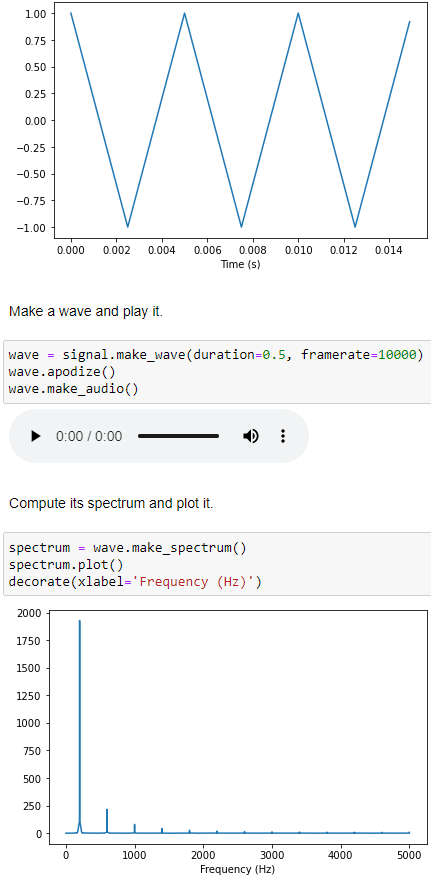
\includegraphics[width=0.55\linewidth]{resources/Images/task1_check_triangle}
        \caption{Изучение и проверка примеров (треугольный сигнал).}
        \label{fig:task1_check_triangle}
    \end{figure}

    \begin{figure}[H]
        \centering
        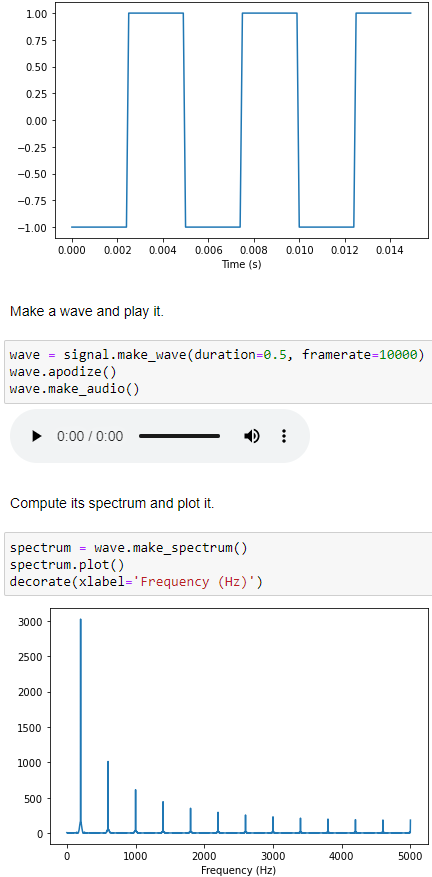
\includegraphics[width=0.6\linewidth]{resources/Images/task1_check_square}
        \caption{Изучение и проверка примеров (прямоугольный сигнал).}
        \label{fig:task1_check_square}
    \end{figure}

    \begin{figure}[H]
        \centering
        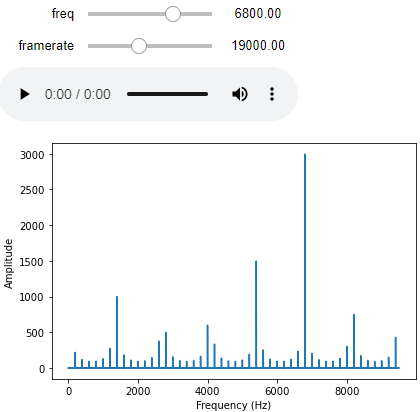
\includegraphics[width=0.8\linewidth]{resources/Images/task1_check_aliasing}
        \caption{Изучение и проверка примеров (влияние эффекта \texttt{aliasing}).}
        \label{fig:task1_check_aliasing}
    \end{figure}

    Все примеры были изучены и запущены.

    В ходе выполнения данного упражнения были получены знания по созданию различных видов сигналов и работе с ними с помощью библиотеки для Python.
    Также было прослушаны звучания этих видов сигналов. Самым приятным из них на слух показался треугольный сигнал.
    Кроме того был рассмотрен эффект \texttt{aliasing}, из-за которого выборки из сигнала с высокой частотой кажутся выборками из сигнала с низкой.
    Были также рассмотрены примеры работы с фазой.

    \newpage

% ---------------------------------------------- Упражнение 2.2 ----------------------------------------------
    \section{Упражнение 2.2}
    \label{sec:task2}

    Во втором упражнении необходимо написать класс \texttt{SawtoothSignal}, расширяющий \texttt{signal} и предоставляющий \texttt{evaluate} для оценки пилообразного сигнала.
    Затем необходимо вычислить спектр пилообразного сигнала и соотнести его гармоническую структуру с треугольным и прямоугольным сигналами.

    Итак, начнём с написания класса \texttt{SawtoothSignal}.

    \begin{lstlisting}[caption= Создание класса \texttt{SawtoothSignal}., label={lst:task2_create_class}]
import numpy
from thinkdsp import decorate, Sinusoid, normalize, unbias, SquareSignal, \
    TriangleSignal, SinSignal

class SawtoothSignal (Sinusoid):
    def evaluate(self, ts):
        cycles = self.freq * ts + self.offset / numpy.pi / 2
        frac, _ = numpy.modf(cycles)
        ys = normalize(unbias(frac), self.amp)
        return ys
    \end{lstlisting}

    Данный класс расширяет класс \texttt{Sinusoid} (который, в свою очередь, расширяет класс \texttt{Signal}) и переопределяет его метод \texttt{evaluate}.

    Теперь проверим работу нашего класса, создав пилообразный сигнал. Затем преобразуем его к \texttt{wave} и выведем график его небольшого сегмента, чтобы увидеть поведение сигнала.
    Тут же прослушаем полученный сигнал.

    \begin{lstlisting}[caption= Работа с пилообразным сигналом., label={lst:task2_work_with_swatooth}]
sawtooth_signal = SawtoothSignal()
sawtooth_wave = sawtooth_signal.make_wave(duration=0.5, framerate=60000)
sawtooth_wave.segment(start=0, duration=sawtooth_signal.period*4).plot()
decorate(xlabel='Time (s)')
sawtooth_wave.make_audio()
    \end{lstlisting}

    Как видно из Рис.\ref{fig:task2_segment_signal}, полученный сигнал действительно пилообразный.
    Это означает, что написанный нами класс работает корректно. Полученный же звук напоминает резкий и неприятный гудок.

    Теперь вычислим спектр полученного пилообразного сигнала.

    \begin{lstlisting}[caption= Вычисление и вывод спектра пилообразного сигнала., label={lst:task2_spectrum_sawtooth}]
sawtooth_wave.make_spectrum().plot()
decorate(xlabel='Frequency (Hz)', ylabel='Amplitude')
    \end{lstlisting}

    \begin{figure}[H]
        \centering
        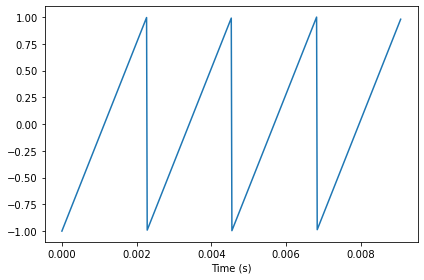
\includegraphics[width=0.8\linewidth]{resources/Images/task2_segment_signal}
        \caption{Сегмент полученного сигнала.}
        \label{fig:task2_segment_signal}
    \end{figure}

    \begin{figure}[H]
        \centering
        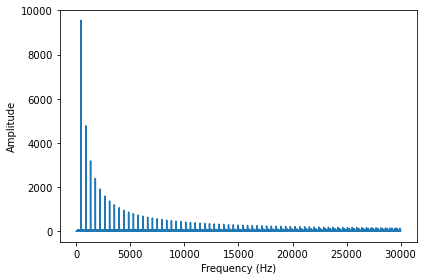
\includegraphics[width=0.8\linewidth]{resources/Images/task2_spectrum_sawtooth}
        \caption{Спектр пилообразного сигнала.}
        \label{fig:task2_spectrum_sawtooth}
    \end{figure}

    Далее сопоставим спектры пилообразного и треугольного сигналов.
    Для этого создадим треугольный сигнал и преобразуем его к \texttt{wave}, после чего выведем его спектр вместе со спектром пилообразного сигнала.

    \begin{lstlisting}[caption= Вывод спектров треугольного и пилообразного сигналов., label={lst:task2_spectrum_sawtooth_triangle}]
sawtooth_wave.make_spectrum().plot(color='red')
triangle_wave = TriangleSignal(amp=0.79).make_wave(duration=0.5, framerate=60000)
triangle_wave.make_audio()
triangle_wave.make_spectrum().plot(color='blue')
decorate(xlabel='Frequency (Hz)', ylabel='Amplitude')
    \end{lstlisting}

    \begin{figure}[h]
        \centering
        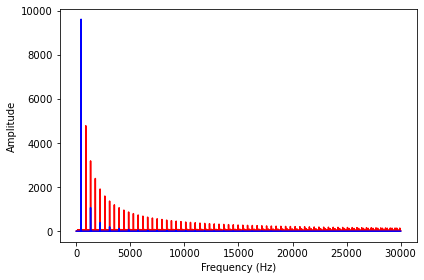
\includegraphics[width=0.8\linewidth]{resources/Images/task2_spectrum_sawtooth_triangle}
        \caption{Спектры пилообразного (красный) и треугольного (синий) сигналов.}
        \label{fig:task2_spectrum_sawtooth_triangle}
    \end{figure}

    Как видно из Рис.\ref{fig:task2_spectrum_sawtooth_triangle}, пилообразный сигнал уменьшается медленнее, чем треугольный.
    Гармоники треугольного сигнала убывают пропорционально $1/f^2$, а пилообразного как $1/f$.
    Звук же треугольного сигнала по сравнению с пилообразным более мягкий, без резких высоких частот.

    Теперь сравним спектры пилообразного и прямоугольного сигналов.

    \begin{lstlisting}[caption= Вывод спектров прямоугольного и пилообразного сигналов., label={lst:task2_spectrum_sawtooth_square}]
sawtooth_wave.make_spectrum().plot(color='red')
square_wave = SquareSignal(amp=0.5).make_wave(duration=0.5, framerate=60000)
square_wave.make_audio()
square_wave.make_spectrum().plot(color='blue')
decorate(xlabel='Frequency (Hz)', ylabel='Amplitude')
    \end{lstlisting}

    \begin{figure}[H]
        \centering
        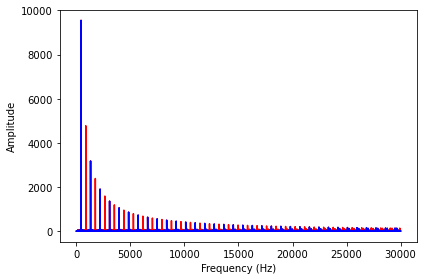
\includegraphics[width=0.8\linewidth]{resources/Images/task2_spectrum_sawtooth_square}
        \caption{Спектры пилообразного (красный) и прямоугольного (синий) сигналов.}
        \label{fig:task2_spectrum_sawtooth_square}
    \end{figure}

    Как видно из Рис.\ref{fig:task2_spectrum_sawtooth_square}, спектры пилообразного и прямоугольного сигналов уменьшаются одинаково,
    но пилообразный включает в себя чётные и нечётные гармоники (это хорошо заметно при сравнении Рис.\ref{fig:task2_spectrum_sawtooth_square} и Рис.\ref{fig:task2_spectrum_sawtooth}).
    Звук же прямоугольного сигнала по сравнению с пилообразным кажется более низким и приглушённым.

    В ходе выполнения данного задания был описан класс \texttt{SawtoothSignal}, формирующий пилообразный сигнал.
    Работа класса была проверена, был сделан вывод, что она работает корректно.
    Затем спектр сформированного пилообразного сигнала был сравнён со спектрами треугольного и прямоугольного сигналов.
    Был сделан вывод, что гармоники треугольного сигнала убывают как $1/f^2$, а пилообразного как $1/f$.
    А также, что спектры пилообразного и прямоугольного сигналов уменьшаются одинаково, но пилообразный включает в себя чётные и нечётные гармоники.

    \newpage

% ---------------------------------------------- Упражнение 2.3 ----------------------------------------------
    \section{Упражнение 2.3}
    \label{sec:task3}

    В этом упражнении необходимо создать прямоугольный сигнал 1100 Гц, вычислить его \texttt{wave} с выборками 10000 кадров в секунду.
    Затем необходимо построить спектр и убедиться, что большинство гармоник "завёрнуты" из-за биений.

    Итак, начнём с создания прямоугольного сигнала заданной частоты. Затем вычислим его \texttt{wave} с выборками 10000 кадров в секунду,
    после чего выведем его спектр (Рис.\ref{fig:task3_spectrum}).

    \begin{lstlisting}[caption= Создание сигнала и получение его \texttt{wave}., label={lst:task3_create_and_spectrum}]
square_wave = SquareSignal(1100).make_wave(duration=0.5, framerate=10000)
square_wave.make_spectrum().plot()
decorate(xlabel='Frequency (Hz)', ylabel='Amplitude')
    \end{lstlisting}

    \begin{figure}[H]
        \centering
        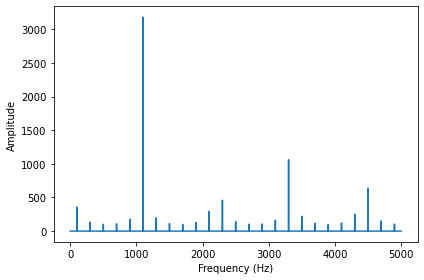
\includegraphics[width=0.8\linewidth]{resources/Images/task3_spectrum}
        \caption{Спектр прямоугольного сигнала.}
        \label{fig:task3_spectrum}
    \end{figure}

    Мы уже знаем, что прямоугольный сигнал содержит только нечётные гармоники.
    Таким образом, ожидалось увидеть гармоники на частотах 1100, 3300, 5500, 7700 и 9900 Гц.
    А теперь внимательно изучим Рис.\ref{fig:task3_spectrum}. Как и ожидалось, пики есть на 1100 и 3300 Гц, но третий пик
    находится на 4500, а не на 5500 Гц. Четвёртый же пик находится на 2300, а не на 7700 Гц, а пятый - на 100, а не на 9900 Гц.

    Подобное поведение возникает из-за эффекта биений.
    Самой высокой частотой, которую можно обработать, могла бы быть 5000 Гц (половина частоты дискретизации), а в нашем же случае - 3300 Гц.
    Частоты выше 5000 Гц "заворачиваются" вокруг 5000 Гц (частота заворота).
    Именно поэтому мы видим ожидаемые пики на 1100 и 3300 Гц, а все остальные "заворачиваются" из-за биений.

    Теперь узнаем, слышны ли последствия этого эффекта при проигрывании.
    Для этого сначала преобразуем \texttt{wave} нашего сигнала в аудио и прослушаем.

    \begin{lstlisting}[caption= Преобразование в аудио., label={lst:task3_audio_square}]
square_wave.make_audio()
    \end{lstlisting}

    Также мы уже знаем, что воспринимаемые тон и высота звука обычно определяются основной частотой (компонента с самой низкой частотой),
    в нашем же случае это 100 Гц ("завёрнутая" четвёртая по счёту гармоника).
    А потому сравним полученный звук с синусоидой 100 Гц.

    \begin{lstlisting}[caption= Получение аудио синусоиды 100 Гц., label={lst:task3_audio_sin}]
SinSignal(100).make_wave(duration=0.5, framerate=10000).make_audio()
    \end{lstlisting}

    Конечно, эти два звука не одинаковы. В первом (прямоугольный сигнал) очень заметен высокий звук, во втором (синусоида) же его нет.
    Однако, можно заметить, что именно фоновый "гул" с первой записи воспринимается схожим со второй записью.

    В ходе выполнения данного упражнения был создан прямоугольный сигнал 1100 Гц, затем вычислен его \texttt{wave} с выборками 10000 кадров в секунду.
    После этого был построен спектр, по которому видно, что большинство гармоник "завёрнуты" из-за биений.

    Кроме того, созданный сигнал был преобразован в аудио и сравнён с аудио синусоиды 100 Гц. При их прослушивании слышно,
    что полученные аудио сами по себе и не воспринимаются одинаковыми (или хотя бы похожими), однако фоновый звук первого аудио
    похож на аудио синусоиды. Таким образом, можно сделать вывод, что в данном примере последствия эффекта биения хоть и слышны
    при проигрывании, однако влияют не очень сильно.

    \newpage

% ---------------------------------------------- Упражнение 2.4 ----------------------------------------------
    \section{Упражнение 2.4}
    \label{sec:task4}

    В данном упражнении осуществляется работа с объектом \texttt{Spectrum}.
    При наличии объекта \texttt{Spectrum} мы можем вывести несколько первых значений \texttt{spectrum.fs}.
    В таком случае мы увидим, что они начинаются с нуля, то есть \texttt{spectrum.hs[0]} - амплитуда компоненты с частотой 0.
    Но что это значит? Данное упражнение направлено на получения ответа на этот вопрос и подразумевает проведение эксперимента
    со \texttt{Spectrum}.

    Итак, для начала создадим треугольный сигнал частотой 440 Гц, получим и выведем его \texttt{wave}.

    \begin{lstlisting}[caption= Создание сигнала и получение\texttt{wave}., label={lst:task4_wave}]
triangle_wave = TriangleSignal(440).make_wave(duration=0.01)
triangle_wave.plot()
decorate(xlabel='Time (s)')
    \end{lstlisting}

    \begin{figure}[h]
        \centering
        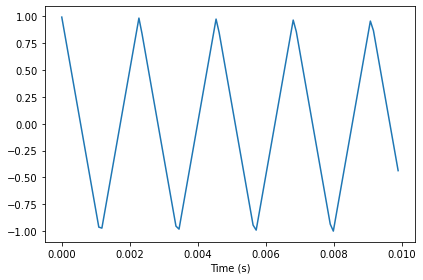
\includegraphics[width=0.8\linewidth]{resources/Images/task4_wave}
        \caption{\texttt{Wave} треугольного сигнала.}
        \label{fig:task4_wave}
    \end{figure}

    Теперь получим спектр и выведем \texttt{spectrum.hs[0]}.

    \begin{lstlisting}[caption= Получение спектра и вывод \texttt{spectrum.hs[0]}., label={lst:task4_spectrum_hs}]
triangle_spectrum = triangle_wave.make_spectrum()
triangle_spectrum.hs[0]
    \end{lstlisting}

    Было получено значение первого элемента спектра (1.0436096431476471e-14+0j). Это комплексное число, близкое к 0.
    Это значение соответствует компоненте нулевой частоты: размах пропорционален амплитуде компоненты,
    а угол - это фаза.

    Теперь установим \texttt{spectrum.hs[0] = 100} и проверим, как это повлияет на сигнал.
    Для этого преобразуем изменённый спектр к \texttt{wave} и сравним его с неизменённым \texttt{wave}.

    \begin{lstlisting}[caption= Изменение первого элемента спектра и сравнение с первоначальным., label={lst:task4_editing_hs_and_copmare}]
triangle_spectrum.hs[0] = 100
triangle_wave.plot(color='blue')
triangle_spectrum.make_wave().plot(color='red')
decorate(xlabel='Time (s)')
    \end{lstlisting}

    \begin{figure}[h]
        \centering
        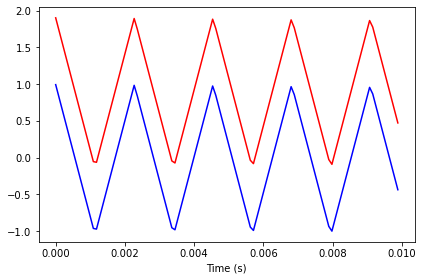
\includegraphics[width=0.8\linewidth]{resources/Images/task4_compare_wave}
        \caption{Сравнение изменённого (красный) и неизменённого (синий) сигналов.}
        \label{fig:task4_compare_wave}
    \end{figure}

    При сравнении можно заметить, что \texttt{wave} вертикально сместилась вверх.
    Такое изменение объясняется тем, что компонент нулевой частоты постоянен для всех значений в сигнале.
    Если сигнал несмещён, то компонент нулевой частоты будет равен 0.
    Таким образом, изменив компоненту нулевой частоты, мы сместили весь сигнал.

    В ходе выполнения данного упражнения был проведён эксперимент со \texttt{Spectrum}.
    В ходе эксперимента была получена и изменена компонента нулевой частоты спектра треугольного сигнала.
    Это привело к смещению \texttt{wave} сигнала. Был сделан вывод, что изменение нулевой компоненты частоты
    влияет на все значения сигнала.

    \newpage

% ---------------------------------------------- Упражнение 2.5 ----------------------------------------------
    \section{Упражнение 2.5}
    \label{sec:task5}

    В данном упражнении необходимо написать функцию, принимающую в качестве параметра \texttt{Spectrum} и изменяющую его
    делением каждого элемента \texttt{hs} на соответствующую частоту из \texttt{fs}. Затем необходимо протестировать написанную функцию.

    Сначала напишем функцию. Не забываем, что на нуль делить не стоит, а потому компоненту нулевой частоты обрабатываем отдельно.

    \begin{lstlisting}[caption= {Функция, изменяющая спектр.}, label={lst:task5_function}]
def change_spectrum(spectrum):
    spectrum.hs[0] = 0
    spectrum.hs[1:] /= spectrum.fs[1:]
    \end{lstlisting}

    Теперь протестируем нашу функцию на пилообразном сигнале. Для этого сначала создадим сигнал, после чего вычислим и распечатаем его спектр.
    Тут же получим аудио нашего сигнала для последующего сравнения.

    \begin{lstlisting}[caption= Создание пилообразного сигнала и получение его спектра., label={lst:task5_spectrum}]
sawtooth_wave = SawtoothSignal().make_wave(duration=0.5)
sawtooth_wave.make_audio()

sawtooth_spectrum = sawtooth_wave.make_spectrum()
sawtooth_spectrum.plot()
decorate(xlabel='Frequency (Hz)', ylabel='Amplitude')
    \end{lstlisting}

    \begin{figure}[H]
        \centering
        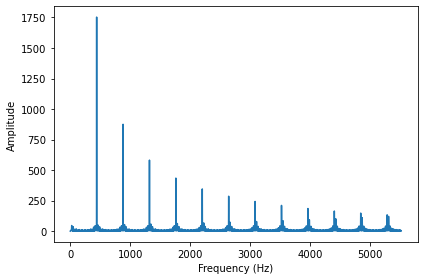
\includegraphics[width=0.7\linewidth]{resources/Images/task5_spectrum}
        \caption{Спектр пилообразного сигнала.}
        \label{fig:task5_spectrum}
    \end{figure}

    Теперь изменим спектр с помощью нашей функции и сравним его с первоначальным спектром.

    \begin{lstlisting}[caption= Изменение спектра и его сравнине с первоначальным спектром., label={lst:task5_compare_spectrum}]
sawtooth_spectrum.plot(color='blue')
change_spectrum(sawtooth_spectrum)
sawtooth_spectrum.scale(440)
sawtooth_spectrum.plot(color='red')
decorate(xlabel='Frequency (Hz)', ylabel='Amplitude')
    \end{lstlisting}

    \begin{figure}[H]
        \centering
        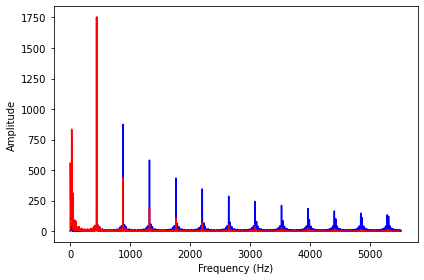
\includegraphics[width=0.8\linewidth]{resources/Images/task5_compare_spectrum}
        \caption{Сравнение изменённого спектра (красный) с первоначальным (синий).}
        \label{fig:task5_compare_spectrum}
    \end{figure}

    Ну и наконец получим аудио из изменённого спектра для сравнения с первоначальным.

    \begin{lstlisting}[caption= Получение аудио., label={lst:task5_new_wave_audio}]
sawtooth_spectrum.make_wave().make_audio()
    \end{lstlisting}

    Полученный сигнал более приглушённый и имеет явно выраженные звуки "бульканья" на фоне.

    В ходе данного упражнения была написана функция, принимающая \texttt{Spectrum} как параметр и изменяющая его
    делением каждого элемента \texttt{hs} на соответствующую частоту из \texttt{fs}.
    Затем эта функция была протестирована на пилообразном сигнале.
    При сравнении звучаний первоначального и изменённого сигналов было замечено, что изменённый сигнал как будто имеет
    более плохое качество: он более тихий и имеет явно выраженные звуки "бульканья" на фоне.

    \newpage

% ---------------------------------------------- Упражнение 2.6 ----------------------------------------------
    \section{Упражнение 2.6}
    \label{sec:task6}

    В этом упражнении предлагается составить сигнал, состоящий из чётных и нечётных гармоник, спадающих пропорционально $1/f^2$.

    Попробуем взять сигнал с необходимым спектром и изменить его параметры для получения необходимого результата.
    Для этого нам подойдёт пилообразный сигнал.

    Итак, создадим сигнал, получим его \texttt{wave} и аудио.

    \begin{lstlisting}[caption= Создание пилообразного сигнала и получение его \texttt{wave}., label={lst:task6_create_wave}]
sawtooth_wave = SawtoothSignal(500).make_wave(duration=0.5, framerate=20000)
sawtooth_wave.make_audio()
    \end{lstlisting}

    Теперь вычислим его спектр и выведем его.

    \begin{lstlisting}[caption= Вычисленине и вывод спектра., label={lst:task6_sawtooth_spectrum}]
sawtooth_spectrum = sawtooth_wave.make_spectrum()
sawtooth_spectrum.plot()
decorate(xlabel='Frequency (Hz)', ylabel='Amplitude')
    \end{lstlisting}

    \begin{figure}[h]
        \centering
        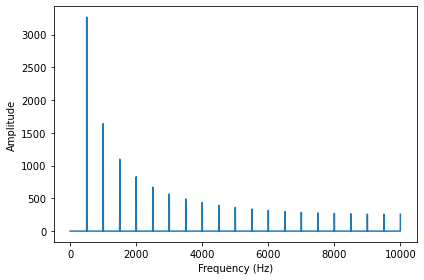
\includegraphics[width=0.8\linewidth]{resources/Images/task6_sawtooth_spectrum}
        \caption{Спектр пилообразного сигнала.}
        \label{fig:task6_sawtooth_spectrum}
    \end{figure}

    Как видно из спектра (Рис.\ref{fig:task6_sawtooth_spectrum}), у нас уже имеются все необходимые гармоники.
    Осталось только изменить спад гармоник с $1/f$ на $1/f^2$. Для этого можно использовать написанную в прошлом
    упражнении функцию \texttt{change\_spectrum()}.

    Итак, изменим спад гармоник и сравним изменённый спектр с первоначальным.

    \begin{lstlisting}[caption= Изменение спада гармоник и сравнение спектров., label={lst:task6_change_and_compare_spectrum}]
sawtooth_spectrum.plot(color='blue')
change_spectrum(sawtooth_spectrum)
sawtooth_spectrum.scale(400)
sawtooth_spectrum.plot(color='red')
decorate(xlabel='Frequency (Hz)', ylabel='Amplitude')
    \end{lstlisting}

    \begin{figure}[h]
        \centering
        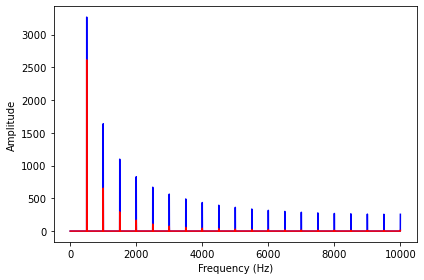
\includegraphics[width=0.8\linewidth]{resources/Images/task6_compare_spectrum}
        \caption{Сравнение спектров пилообразного и полученного сигналов.}
        \label{fig:task6_compare_spectrum}
    \end{figure}

    Как видно из Рис.\ref{fig:task6_compare_spectrum}, теперь гармоники спадают как $1/f^2$.
    Преобразуем изменённый спектр в \texttt{wave}, выведем его сегмент и получим аудио.

    \begin{lstlisting}[caption= Получение аудио и \texttt{wave}., label={lst:task6_wave_and_audio}]
sawtooth_wave_new = sawtooth_spectrum.make_wave()
sawtooth_wave_new.segment(duration=0.01).plot()
decorate(xlabel='Time (s)')
sawtooth_wave_new.make_audio()
    \end{lstlisting}

    \begin{figure}[H]
        \centering
        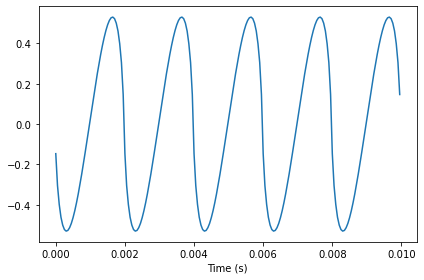
\includegraphics[width=0.8\linewidth]{resources/Images/task6_signal_wave}
        \caption{Сегмент полученного сигнала.}
        \label{fig:task6_signal_wave}
    \end{figure}

    Полученный сигнал имеет как будто промежуточный вид между синусоидой и пилообразным сигналом.
    При этом звучит он гораздо мягче и приятнее, чем первоначальный пилообразный сигнал.

    В ходе выполнения данного упражнения на основе пилообразного сигнала был создан сигнал, состоящий из чётных и
    нечётных гармоник, спадающих пропорционально $1/f^2$. Полученный сигнал звучит мягче и приятнее пилообразного сигнала.

    \newpage

% ------------------------------------------------- Выводы -------------------------------------------------
    \section{Выводы}
    \label{sec:conclusions}

    В ходе выполнения данной лабораторной работы были изучены спектры, гармоники и некоторые виды сигналов: треугольный, прямоугольный и пилообразный.
    Был создан и протестирован класс \texttt{SawtoothSignal}, формирующий пилообразный сигнал.
    Также был изучен и эффект биения, из-за которого происходит "заворот" гармоник. Кроме того, было изучено влияние компоненты нулевой частоты на сигнал.
    Затем была написана и протестирована функция, изменяющая спектр. И наконец, был составлен сигнал согласно требованиям.

\end{document}